%% Elemantary polarization
%% 
%% In header include:
%%   \usepackage{tikz}
%% Usage:
%%   \begin{figure} %% Elemantary polarization
%% 
%% In header include:
%%   \usepackage{tikz}
%% Usage:
%%   \begin{figure} %% Elemantary polarization
%% 
%% In header include:
%%   \usepackage{tikz}
%% Usage:
%%   \begin{figure} %% Elemantary polarization
%% 
%% In header include:
%%   \usepackage{tikz}
%% Usage:
%%   \begin{figure} \input{elementary_polarization.tex} \end{figure}
%
\scalebox{0.9}{
  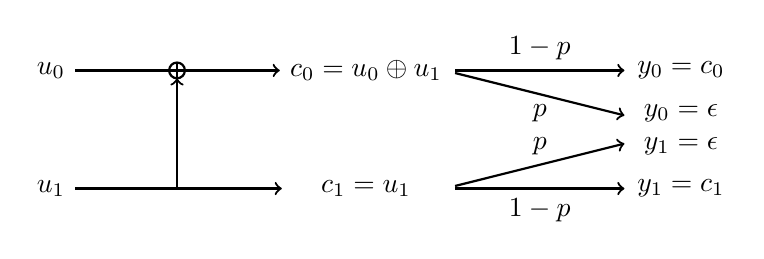
\begin{tikzpicture}[black, thick]
    \newcommand\XL{0}
    \newcommand\XH{4}
    \newcommand\YL{0}
    \newcommand\YH{1.5}
    \newcommand\R{0.1}
    \node (U0) at (\XL, \YH){$u_0$};
    \node (U1) at (\XL, \YL){$u_1$};
    \node[rectangle, minimum width=6em] (C0) at (\XH, \YH){$c_0 = u_0 \oplus u_1$};
    \node[rectangle, minimum width=6em] (C1) at (\XH, \YL){$c_1 = u_1$};
    \node (C0a) at (\XH+1, \YH){};
    \node (C1a) at (\XH+1, \YL){};
    \node[minimum width=4em] (Y0) at (2*\XH, \YH){$y_0 = c_0$};
    \node[minimum width=4em] (Y1) at (2*\XH, \YL){$y_1 = c_1$};
    \node[align=left,minimum width=4em] (E) at (2*\XH, \YH/2){$y_0 = \epsilon$\\$y_1 = \epsilon$};
    \draw[->] (U0) edge (C0) (C0a) edge node[midway, above]{$1-p$} (Y0);
    \draw[->] (U1) edge (C1) (C1a) edge node[midway, below]{$1-p$} (Y1);
    \draw (\XH/2.5, \YH) circle (\R);
    \draw (\XH/2.5, \YH-\R) -- (\XH/2.5, \YH+\R);
    \draw[->] (\XH/2.5, \YL) -- (\XH/2.5, \YH-\R);
    \draw[->] (C0a) edge node[midway, below]{$p$} (E);
    \draw[->] (C1a) edge node[midway, above]{$p$} (E);
  \end{tikzpicture}
}
 \end{figure}
%
\scalebox{0.9}{
  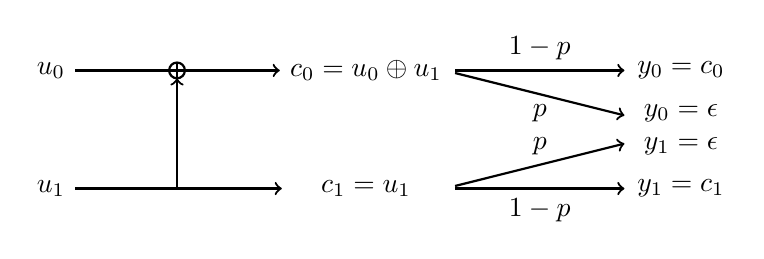
\begin{tikzpicture}[black, thick]
    \newcommand\XL{0}
    \newcommand\XH{4}
    \newcommand\YL{0}
    \newcommand\YH{1.5}
    \newcommand\R{0.1}
    \node (U0) at (\XL, \YH){$u_0$};
    \node (U1) at (\XL, \YL){$u_1$};
    \node[rectangle, minimum width=6em] (C0) at (\XH, \YH){$c_0 = u_0 \oplus u_1$};
    \node[rectangle, minimum width=6em] (C1) at (\XH, \YL){$c_1 = u_1$};
    \node (C0a) at (\XH+1, \YH){};
    \node (C1a) at (\XH+1, \YL){};
    \node[minimum width=4em] (Y0) at (2*\XH, \YH){$y_0 = c_0$};
    \node[minimum width=4em] (Y1) at (2*\XH, \YL){$y_1 = c_1$};
    \node[align=left,minimum width=4em] (E) at (2*\XH, \YH/2){$y_0 = \epsilon$\\$y_1 = \epsilon$};
    \draw[->] (U0) edge (C0) (C0a) edge node[midway, above]{$1-p$} (Y0);
    \draw[->] (U1) edge (C1) (C1a) edge node[midway, below]{$1-p$} (Y1);
    \draw (\XH/2.5, \YH) circle (\R);
    \draw (\XH/2.5, \YH-\R) -- (\XH/2.5, \YH+\R);
    \draw[->] (\XH/2.5, \YL) -- (\XH/2.5, \YH-\R);
    \draw[->] (C0a) edge node[midway, below]{$p$} (E);
    \draw[->] (C1a) edge node[midway, above]{$p$} (E);
  \end{tikzpicture}
}
 \end{figure}
%
\scalebox{0.9}{
  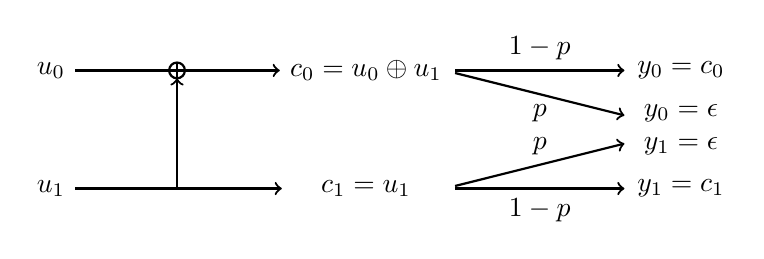
\begin{tikzpicture}[black, thick]
    \newcommand\XL{0}
    \newcommand\XH{4}
    \newcommand\YL{0}
    \newcommand\YH{1.5}
    \newcommand\R{0.1}
    \node (U0) at (\XL, \YH){$u_0$};
    \node (U1) at (\XL, \YL){$u_1$};
    \node[rectangle, minimum width=6em] (C0) at (\XH, \YH){$c_0 = u_0 \oplus u_1$};
    \node[rectangle, minimum width=6em] (C1) at (\XH, \YL){$c_1 = u_1$};
    \node (C0a) at (\XH+1, \YH){};
    \node (C1a) at (\XH+1, \YL){};
    \node[minimum width=4em] (Y0) at (2*\XH, \YH){$y_0 = c_0$};
    \node[minimum width=4em] (Y1) at (2*\XH, \YL){$y_1 = c_1$};
    \node[align=left,minimum width=4em] (E) at (2*\XH, \YH/2){$y_0 = \epsilon$\\$y_1 = \epsilon$};
    \draw[->] (U0) edge (C0) (C0a) edge node[midway, above]{$1-p$} (Y0);
    \draw[->] (U1) edge (C1) (C1a) edge node[midway, below]{$1-p$} (Y1);
    \draw (\XH/2.5, \YH) circle (\R);
    \draw (\XH/2.5, \YH-\R) -- (\XH/2.5, \YH+\R);
    \draw[->] (\XH/2.5, \YL) -- (\XH/2.5, \YH-\R);
    \draw[->] (C0a) edge node[midway, below]{$p$} (E);
    \draw[->] (C1a) edge node[midway, above]{$p$} (E);
  \end{tikzpicture}
}
 \end{figure}
%
\scalebox{0.9}{
  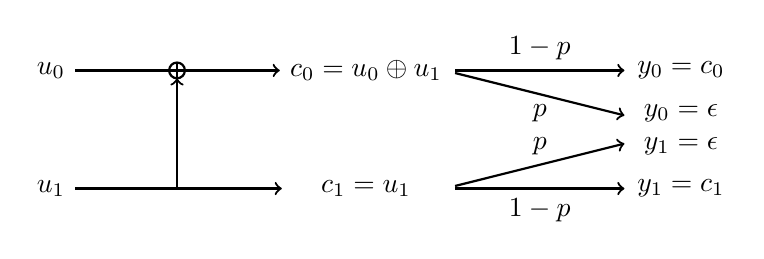
\begin{tikzpicture}[black, thick]
    \newcommand\XL{0}
    \newcommand\XH{4}
    \newcommand\YL{0}
    \newcommand\YH{1.5}
    \newcommand\R{0.1}
    \node (U0) at (\XL, \YH){$u_0$};
    \node (U1) at (\XL, \YL){$u_1$};
    \node[rectangle, minimum width=6em] (C0) at (\XH, \YH){$c_0 = u_0 \oplus u_1$};
    \node[rectangle, minimum width=6em] (C1) at (\XH, \YL){$c_1 = u_1$};
    \node (C0a) at (\XH+1, \YH){};
    \node (C1a) at (\XH+1, \YL){};
    \node[minimum width=4em] (Y0) at (2*\XH, \YH){$y_0 = c_0$};
    \node[minimum width=4em] (Y1) at (2*\XH, \YL){$y_1 = c_1$};
    \node[align=left,minimum width=4em] (E) at (2*\XH, \YH/2){$y_0 = \epsilon$\\$y_1 = \epsilon$};
    \draw[->] (U0) edge (C0) (C0a) edge node[midway, above]{$1-p$} (Y0);
    \draw[->] (U1) edge (C1) (C1a) edge node[midway, below]{$1-p$} (Y1);
    \draw (\XH/2.5, \YH) circle (\R);
    \draw (\XH/2.5, \YH-\R) -- (\XH/2.5, \YH+\R);
    \draw[->] (\XH/2.5, \YL) -- (\XH/2.5, \YH-\R);
    \draw[->] (C0a) edge node[midway, below]{$p$} (E);
    \draw[->] (C1a) edge node[midway, above]{$p$} (E);
  \end{tikzpicture}
}
